\subsection{有限维单 g-模的最高权}

定理 1. 单 g-模是有限维的，当且仅当它具有属于 \(P_{++}\) 的最高权。

以 V 表示一个单 g-模，以 X 表示其权集。

\begin{enumerate}
\def\labelenumi{\alph{enumi})}
\item
  假设 V 是有限维的。于是 X 是有限且非空的（命题 1），因而有一个极大元 \(\omega\)。设 \(\alpha \in B\)。则 \(\omega + \alpha \notin X\)，这证明了 \(\omega\) 是 V 的最高权（§6，第 2 节，引理 2）。另一方面，存在一个从 \(\mathfrak{sl}(2, k)\) 到 g 的同态，将 H 映到 \(H_{\alpha}\)；由 §1，命题 2 (i)，\(\omega(H_{\alpha})\) 是一个 \(\geq 0\) 的整数，所以 \(\omega \in P_{++}\)。
\item
  假设 V 具有最高权 \(\omega\in P_{++}\)。设 \(\alpha\in B\)，并设 e 是 V 中权为 \(\omega\) 的本原元。置 \(e_{j}=X_{-\alpha}^{j}e\)（\(j\geq0\)），\(m=\omega(H_{\alpha})\in N\)，以及 \(N=\sum_{j=0}^{m}ke_{j}\)。根据 §1，第 2 节，命题 1，\(X_{\alpha}e_{m+1}=0\)。若 \(\beta\in B\) 且 \(\beta\neq\alpha\)，则 \([X_{\beta},X_{-\alpha}]=0\)，所以 \(X_{\beta}e_{m+1}=X_{\beta}X_{-\alpha}^{m+1}e=X_{-\alpha}^{m+1}X_{\beta}e=0\)。如果 \(e_{m+1}\neq0\)，我们便得到 \(e_{m+1}\) 是本原元，这不可能（§6，命题 3 (i)）；因此 \(e_{m+1}=0\)。于是，根据 §1，第 2 节，命题 1 的推论，N 在子代数 \(s_{\alpha}\) 下稳定；该子代数由 \(H_{\alpha},X_{\alpha}\) 和 \(X_{-\alpha}\) 生成。现在 \(s_{\alpha}\) 在 g 中是约化的，因此 V 中在 \(s_{\alpha}\) 下稳定的有限维子空间之和是 V 的一个 g-子模（第 I 章，§6，第 6 节，命题 7）；由于这个和非零，它等于 V。由此可知 \((X_{\alpha})_{V}\) 和 \((X_{-\alpha})_{V}\) 是局部幂零的。根据引理 1 (ii)，X 在 \(s_{\alpha}\) 下稳定，并且这对所有 \(\alpha\) 都成立。因此 X 在 W 下稳定。现在 W 在 P 上的每个轨道都与 \(P_{++}\) 相交（第 VI 章，§1，第 10 节）。另一方面，如果 \(\lambda\in X\cap P_{++}\)，则 \(\lambda=\omega-\sum_{\alpha\in B}n_{\alpha}\alpha=\sum_{\alpha\in B}n'_{\alpha}\alpha\)，其中 \(n_{\alpha}\in N\)，并且 \(n'_{\alpha}\geq0\) 对所有 \(\alpha\in B\) 成立（第 V 章，§3，第 5 节，引理 6）。所以 \(X\cap P_{++}\) 是有限的，因而 X 也是有限的。由于每个权的重数都是有限的（§6，第 1 节，命题 1 (ii)），V 是有限维的。
\end{enumerate}

推论 1. 若 \(\lambda \in \mathfrak{h}^*\) 且 \(\lambda \notin \mathrm{P}_{++}\)，则 \(\mathfrak{g}\)-模 \(\mathrm{E}(\lambda)\)（§6，第 3 节）是无限维的。

推论 2. g-模 \(E(\lambda)\)（其中 \(\lambda \in P_{++}\)）构成有限维单 g-模各同构类的一个代表系。

g-模 \(E(\lambda)\)，其中 \(\lambda\) 是基本权，称为基本 g-模；相应的表示称为 g 的基本表示；它们是绝对不可约的（\(\S6\)，第 2 节，命题 3 (iv)）。

若 V 是有限维 g-模且 \(\lambda\in P_{++}\)，则 V 中类型为 \(\mathrm{E}(\lambda)\) 的同构型分支称为 V 中最高权为 \(\lambda\) 的同构型分支。

备注 1. 设 \(\lambda \in \mathrm{P}_{++}\)，\(\rho_{\lambda}\) 为 \(\mathfrak{g}\) 在 \(\operatorname{E}(\lambda)\) 上的表示，\(s \in \operatorname{Aut}(\mathfrak{g})\)，而 \(\sigma\) 为 \(s\) 在 \(\operatorname{Aut}(\mathrm{R},\mathrm{B})\) 中的典则像（\(\S 5\)，第 3 节，命题 5 的推论 1）。则 \(\rho_{\lambda} \circ s\) 与 \(\rho_{\sigma \lambda}\) 等价；事实上，若 \(s \in \operatorname{Aut}_0(\mathfrak{g})\)，则 \(\rho_{\lambda} \circ s\) 和 \(\rho_{\sigma \lambda}\) 都与 \(\rho_{\lambda}\) 等价（命题 2）；而若 \(s\) 使 \(\mathfrak{h}\) 和 B 保持不变，则 \(\rho_{\lambda} \circ s\) 是最高权为 \(\sigma \lambda\) 的单表示。

特别地，基本表示在 \(s\) 下相互置换，并且这个置换是恒等置换，当且仅当 \(s \in \mathrm{Aut}_0(\mathfrak{g})\)。

命题 3. 设 V 是有限维 g-模，X 是其权集。设 \(\lambda \in X\)，\(\alpha \in R\)，令 I 为满足 \(t \in Z\) 且 \(\lambda + t\alpha \in X\) 的参数所成的集合，p（分别为 -q）为 I 的最大（分别为最小）元素。设 \(m_t\) 是 \(\lambda + t\alpha\) 的重数。

\begin{enumerate}
\def\labelenumi{(\roman{enumi})}
\item
  I = \(\{-q, p\}\)，且 \(q - p = \lambda(H_{\alpha})\)。
\item
  对任意整数 \(u \in [0, p + q]\)，\(\lambda + (p - u)\alpha\) 与 \(\lambda + (-q + u)\alpha\) 在 \(s_{\alpha}\) 下共轭，且 \(m_{-q + u} = m_{p - u}\)。
\item
  若 \(t \in \mathbf{Z}\) 且 \(t < (p - q)/2\)，则 \((X_{\alpha})_{\mathrm{V}}\) 将 \(V^{\lambda + t\alpha}\) 单射地映入 \(V^{\lambda + (t + 1)\alpha}\)。
\item
  函数 \(t \mapsto m_t\) 在 \([-q, (p - q)/2]\) 上递增，在 \([(p - q)/2, p]\) 上递减。
\end{enumerate}

设 \(\alpha \in \mathrm{B}\)。利用 \(\mathfrak{sl}(2,k)\) 中的元素 \(X_{\alpha}, X_{-\alpha}, H_{\alpha}\)，这些元素属于 \(\mathfrak{g}\)，把 V 看作一个模。于是 \(\mathrm{V}^{\lambda + p\alpha}\) 的每个非零元素都是本原元。因此，\((\lambda + p\alpha)(H_{\alpha}) \geq 0\)，并且 \((X_{-\alpha})^{r}\mathrm{V}^{\lambda + p\alpha} \neq 0\) 对于

\[
0 \leq r \leq (\lambda + p \alpha) (H _ {\alpha}) = \lambda (H _ {\alpha}) + 2 p
\]

\pandocbounded{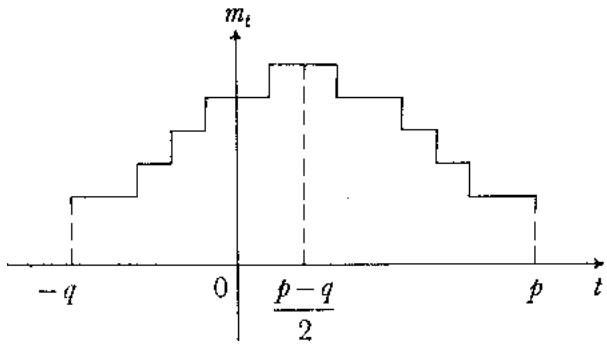
\includegraphics[keepaspectratio]{images/part001_39d2730e.jpg}}

（§1，第 2 节，命题 2）。由此可得：\(\mathrm{V}^{\lambda + t\alpha} \neq 0\)，只要 \(p \geq t \geq p - (\lambda(H_{\alpha}) + 2p)\)，所以 \(p + q \geq \lambda(H_{\alpha}) + 2p\)。将这个结果应用于 \(-\alpha\)，得到

\[
p + q \geq \lambda (H _ {- \alpha}) + 2 q = - \lambda (H _ {\alpha}) + 2 q.
\]

因此 \(q - p = \lambda (H_{\alpha})\)，且 \(\lambda + t\alpha \in \mathcal{X}\)（当 \(p \geq t \geq -q\) 时），这证明了 (i)。

我们有 \(s_{\alpha}(\alpha) = -\alpha\)，且 \(s_{\alpha}(\mu) \in \mu + k\alpha\) 对所有 \(\mu \in \mathfrak{h}^*\) 成立。由于 W 使 \(\mathcal{X}\) 保持稳定（命题 2 的推论 2），\(s_{\alpha}\) 使 \(\{\lambda - q\alpha, \lambda - q\alpha + \alpha, \ldots, \lambda + p\alpha\}\) 保持稳定，并将 \(\lambda - q\alpha + u\alpha\) 映到 \(\lambda + p\alpha - u\alpha\)，其中对所有 \(u \in k\) 都成立。再次使用命题 2 的推论 2，可见 \(m_{-q + u} = m_{p - u}\)，其中 \(u \in [0, p + q]\) 为任意整数。这证明了 (ii)。

根据 §1，命题 2 的推论，\((X_{\alpha})_{\mathrm{V}}|\mathrm{V}^{\lambda +t\alpha}\) 在 \(t < (p - q) / 2\) 时是单射。现在 \((X_{\alpha})_{\mathrm{V}}\) 将 \(\mathrm{V}^{\lambda +t\alpha}\) 映到 \(\mathrm{V}^{\lambda +(t + 1)\alpha}\)。所以 \(m_{t + 1}\geq m_t\)，只要 \(t < (p - q) / 2\)。将 \(\alpha\) 换成 \(-\alpha\)，可见 \(m_{t + 1}\leq m_t\)，只要 \(t > (p - q) / 2\)。这证明了 (iii) 和 (iv)。

推论 1. 若 \(\lambda \in \mathcal{X}\) 且 \(\lambda (H_{\alpha})\geq 1\)，则 \(\lambda -\alpha \in \mathcal{X}\)。若 \(\lambda +\alpha \in \mathcal{X}\) 且 \(\lambda (H_{\alpha}) = 0\)，则 \(\lambda \in \mathcal{X}\) 且 \(\lambda -\alpha \in \mathcal{X}\)。

这立即由命题 3 (i) 得出。

推论 2. 设 \(\mu \in \mathrm{P}_{++}\) 且 \(\nu \in \mathrm{Q}_{+}\)。若 \(\mu + \nu \in \mathcal{X}\)，则 \(\mu \in \mathcal{X}\)。

写成 \(\nu = \sum_{\alpha \in \mathrm{B}} c_{\alpha}.\alpha\)，其中 \(c_{\alpha} \in \mathbf{N}\) 对所有 \(\alpha \in \mathrm{B}\) 成立。当 \(\sum_{\alpha \in \mathrm{B}} c_{\alpha} = 0\) 时推论显然成立；假设 \(\sum_{\alpha \in \mathrm{B}} c_{\alpha} > 0\)，并对 \(\sum_{\alpha \in \mathrm{B}} c_{\alpha}\) 作归纳。设 \((\cdot|\cdot)\) 是 \(\mathfrak{h}_{\mathbf{R}}^{*}\) 上 W-不变的非退化正对称双线性型。于是 \((\nu|\sum_{\alpha \in \mathrm{B}} c_{\alpha}.\alpha) > 0\)，所以存在 \(\beta \in \mathrm{B}\)，使得 \(c_{\beta} \geq 1\) 且 \((\nu|\beta) > 0\)，从而 \(\nu(H_{\beta}) \geq 1\)。由于 \(\mu \in \mathrm{P}_{++}\)，可得 \((\mu + \nu)(H_{\beta}) \geq 1\)。根据推论 1，\(\mu + (\nu - \beta) \in \mathcal{X}\)，于是只需应用归纳假设。

推论 3. 设 \(v \in V\) 是权为 \(\omega\) 的本原元。设 \(\Sigma\) 为满足 \(\alpha \in B\) 且 \(\omega(H_{\alpha}) = 0\) 的元素所成的集合。\(\mathfrak{g}\) 中直线 \(kv\) 的稳定子是抛物子代数 \(\mathfrak{p}_{\Sigma}\)，它对应于 \(\Sigma\)（§3，第 4 节，备注）。

必要时以 v 生成的 g-子模替换 V，于是可假设 V 是单模。设 s 为稳定子。我们有 \((\mathfrak{n}_{+})_{\mathrm{V}}v = 0\)，\((\mathfrak{h})_{\mathrm{V}}v \subset kv\)。设 \(\alpha \in B\) 满足 \(\omega(H_{\alpha}) = 0\)。我们有 \(\omega + \alpha \notin X\)，从而 \(\omega - \alpha \notin X\)（命题 3 (i)），因而 \((\mathfrak{g}^{-\alpha})_{\mathrm{V}}v = 0\)。前述结果说明 \(p_{\Sigma} \subset s\)。若 \(p_{\Sigma} \neq s\)，则 \(s = p_{\Sigma'}\)，其中 \(\Sigma'\) 是严格包含 \(\Sigma\) 的 B 的子集。设 \(\beta \in \Sigma' - \Sigma\)。于是 \(g^{-\beta}\) 稳定 kv，因而湮灭 v。但是，由于 \(\omega(H_{\beta}) > 0\)，这与命题 3 (iii) 矛盾。证毕。

P 的一个子集 \(\mathcal{X}\) 称为 R-饱和的，如果满足以下条件：对所有 \(\lambda \in \mathcal{X}\) 和所有 \(\alpha \in \mathrm{R}\)，有 \(\lambda - t\alpha \in \mathcal{X}\)，其中 \(t\) 遍历 0 与 \(\lambda(H_{\alpha})\) 之间的所有整数。由于 \(s_{\alpha}(\lambda) = \lambda - \lambda(H_{\alpha})\alpha\)，可见 P 的 R-饱和子集在 W 下稳定。设 \(\mathcal{Y} \subset \mathrm{P}\)。\(\lambda\) 是 \(\mathcal{Y}\) 的一个元素，在 \(\mathcal{Y}\) 中称为 R-极值元，如果对所有 \(\alpha \in \mathrm{R}\)，都有 \(\lambda + \alpha \notin \mathcal{Y}\) 或 \(\lambda - \alpha \notin \mathcal{Y}\)。

命题 4. 设 \(\mathrm{V}\) 是有限维 \(\mathfrak{g}\)-模，\(d\) 是满足 \(\geq 1\) 的整数。\(\mathrm{V}\) 中重数 \(\geq d\) 的权的集合是 R-饱和的。

这立即由命题 3 得出。

命题 5. 设 V 是有限维单 g-模，\(\omega\) 是其最高权，X 是其权集。取双线性型 \((\cdot|\cdot)\)，它定义在 \(h_{R}^{*}\) 上，且 W-不变、非退化、正定；并令 \(\lambda\mapsto\|\lambda\|=(\lambda|\lambda)^{1/2}\) 为相应的范数。

\begin{enumerate}
\def\labelenumi{(\roman{enumi})}
\item
  \(\mathcal{X}\) 是包含 \(\omega\) 的 P 的最小 R-饱和子集。
\item
  \(\mathcal{X}\) 的 R-极值元正是 \(\omega\) 在 W 下的变换。
\item
  若 \(\mu \in \mathcal{X}\)，则 \(\| \mu \| \leq \| \omega \|\)。此外，若 \(\mu \neq \omega\)，则 \(\| \mu + \rho \| < \| \omega + \rho \|\)。若 \(\mu\) 不是 \(\mathcal{X}\) 中的 R-极值元，则 \(\| \mu \| < \| \omega \|\)。
\item
  我们有 \(\mathcal{X} = \mathrm{W.}(\mathcal{X}\cap \mathrm{P}_{++})\)。其中，\(\lambda\) 是 \(\mathrm{P}_{++}\) 中的元素；其属于 \(\mathcal{X}\cap \mathrm{P}_{++}\) 当且仅当 \(\omega -\lambda \in \mathrm{Q}_{+}\)。
\item
  设 \(\mathcal{X}'\) 是包含 \(\omega\) 的 P 的最小 R-饱和子集。我们有 \(\mathcal{X}' \subset \mathcal{X}\)（命题 4）。假设 \(\mathcal{X} \neq \mathcal{X}'\)。设 \(\lambda\) 是 \(\mathcal{X} - \mathcal{X}'\) 的极大元。由于 \(\lambda \neq \omega\)，存在 \(\alpha \in B\)，使得 \(\lambda + \alpha \in \mathcal{X}\)。按命题 3 引入 \(p\) 和 \(q\)。由于 \(\lambda\) 是 \(\mathcal{X} - \mathcal{X}'\) 中的极大元，\(\lambda + p\alpha \in \mathcal{X}'\)。根据命题 3 (ii)，\(\lambda - q\alpha \in \mathcal{X}'\)，因为 \(\mathcal{X}'\) 在 W 下稳定。因此，有 \(\lambda + u\alpha \in \mathcal{X}'\)，其中 \(u\) 遍历区间 \([-q, p]\) 中的每个整数。这与 \(\lambda \notin \mathcal{X}'\) 矛盾，从而证明了 (i)。
\item
  显然，\(\omega\) 是 \(\mathcal{X}\) 中的 R-极值元；因此它在 W 下的变换也都是 \(\mathcal{X}\) 中的 R-极值元。设 \(\lambda\) 是 \(\mathcal{X}\) 中的 R-极值元；我们将证明 \(\lambda \in \mathrm{W}.\omega\)。由于存在 \(w \in \mathrm{W}\)，使得 \(w\lambda \in \mathrm{P}_{++}\)（第 VI 章，§1，第 10 节），不妨设 \(\lambda \in \mathrm{P}_{++}\)。设 \(\alpha \in \mathrm{B}\)；按命题 3 引入 \(p\) 和 \(q\)。由于 \(\lambda\) 是 R-极值元，\(p = 0\) 或 \(q = 0\)。由于
\end{enumerate}

\[
q - p = \lambda (H _ {\alpha}) \geq 0,
\]

不可能有 \(p > 0\)。因此 \(p = 0\) 且 \(\lambda = \omega\)。

\begin{enumerate}
\def\labelenumi{(\roman{enumi})}
\setcounter{enumi}{2}
\tightlist
\item
  设 \(\mu \in \mathcal{X} \cap \mathrm{P}_{++}\)。则 \(\omega + \mu \in \mathrm{P}_{++}\) 且 \(\omega - \mu \in \mathrm{Q}_+\)（§6，第 1 节，命题 1），所以 \(0 \leq (\omega - \mu|\omega + \mu) = (\omega|\omega) - (\mu|\mu)\)；从而 \((\mu|\mu) \leq (\omega|\omega)\)，利用 Weyl 群可将此结论推广到所有 \(\mu \in \mathcal{X}\)。如果 \(\mu \in \mathcal{X} - \{\omega\}\)，
\end{enumerate}

\[
\begin{array}{c} (\mu + \rho | \mu + \rho) = (\mu | \mu) + 2 (\mu | \rho) + (\rho | \rho) \leq (\omega | \omega) + 2 (\mu | \rho) + (\rho | \rho) \\ = (\omega + \rho | \omega + \rho) - 2 (\omega - \mu | \rho). \end{array}
\]

现在 \(\omega - \mu = \sum_{\alpha \in \mathrm{B}} n_{\alpha} \alpha\)，其中整数 \(n_{\alpha} \geq 0\) 不全为零，所以 \((\omega - \mu | \rho) > 0\)，因为 \((\rho | \alpha) > 0\) 对所有 \(\alpha \in \mathrm{B}\) 都成立（第 VI 章，§1，第 10 节，命题 29 (iii)）。若 \(\mu\) 不是 \(\mathcal{X}\) 中的 R-极值元，则存在 \(\alpha \in \mathrm{R}\)，使得 \(\mu + \alpha \in \mathcal{X}\) 且 \(\mu - \alpha \in \mathcal{X}\)；于是

\[
\| \mu \| <   \sup (\| \mu + \alpha \|, \| \mu - \alpha \|) \leq \sup _ {\lambda \in \mathcal {X}} \| \lambda \|
\]

而根据前述结果，这个上界是 \(\|\omega\|\)。

\begin{enumerate}
\def\labelenumi{(\roman{enumi})}
\setcounter{enumi}{3}
\tightlist
\item
  根据第 VI 章，§1，第 10 节，我们有 \(\mathcal{X} = \mathrm{W.}(\mathcal{X}\cap \mathrm{P}_{++})\)。若 \(\lambda \in \mathcal{X}\)，则 \(\omega -\lambda \in \mathrm{Q}_{+}\)（§6，第 1 节，命题 1）。若 \(\lambda \in \mathrm{P}_{++}\) 且 \(\omega -\lambda \in \mathrm{Q}_{+}\)，则 \(\lambda \in \mathcal{X}\)（命题 3 的推论 2）。
\end{enumerate}

推论。设 X 是 P 的有限 R-饱和子集。存在一个权集为 X 的有限维 g-模。

由于 \(\mathcal{X}\) 在 W 下稳定，\(\mathcal{X}\) 是包含 \(\mathcal{X} \cap \mathrm{P}_{++}\) 的最小 R-饱和集。根据命题 5 (i)，\(\mathcal{X}\) 是 \(\bigoplus_{\lambda \in \mathcal{X} \cap \mathrm{P}_{++}} \mathrm{E}(\lambda)\) 的权集。

备注 2. 回顾一下（第 VI 章，§1，第 6 节，命题 17 的推论 3），存在唯一的 \(w_0\)，它是 \(\mathrm{W}\) 中将 \(\mathrm{B}\) 变为 \(-\mathrm{B}\) 的元素；我们有 \(w_0^2 = 1\)。并且 \(-w_0\) 保持 \(\mathrm{P}\) 上的序关系。记 \(\mathrm{V}\) 为有限维单 \(\mathfrak{g}\)-模，\(\omega\) 为其最高权。则 \(w_0(\omega)\) 是 \(\mathrm{V}\) 的最低权，且其重数为 1。

